\documentclass[tikz,border=5pt]{standalone}
\usetikzlibrary{shapes.geometric, arrows}

\tikzstyle{input} = [rectangle, rounded corners, minimum width=3cm, minimum height=1cm,text centered, draw=black, fill=blue!20]
\tikzstyle{output} = [rectangle, rounded corners, minimum width=3cm, minimum height=1cm,text centered, draw=black, fill=red!20]
\tikzstyle{process} = [rectangle, minimum width=3cm, minimum height=1cm, text centered, draw=black, fill=orange!20]
\tikzstyle{arrow} = [thick,->,>=stealth]

\begin{document}

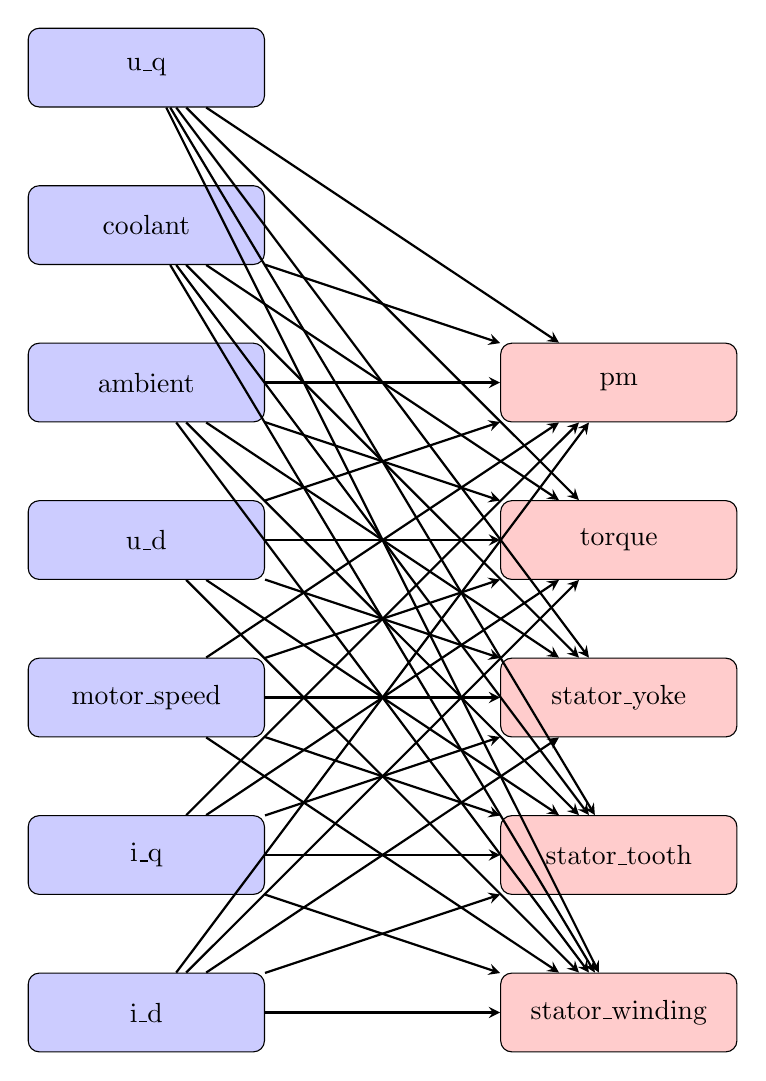
\begin{tikzpicture}[node distance=2cm]

\node (input1) [input] {u\_q};
\node (input2) [input, below of=input1] {coolant};
\node (input3) [input, below of=input2] {ambient};
\node (input4) [input, below of=input3] {u\_d};
\node (input5) [input, below of=input4] {motor\_speed};
\node (input6) [input, below of=input5] {i\_q};
\node (input7) [input, below of=input6] {i\_d};

\node (output1) [output, right of=input4, xshift=4cm] {torque};
\node (output2) [output, above of=output1] {pm};
\node (output3) [output, below of=output1] {stator\_yoke};
\node (output4) [output, below of=output3] {stator\_tooth};
\node (output5) [output, below of=output4] {stator\_winding};

\draw [arrow] (input1) -- (output1);
\draw [arrow] (input1) -- (output2);
\draw [arrow] (input1) -- (output3);
\draw [arrow] (input1) -- (output4);
\draw [arrow] (input1) -- (output5);

\draw [arrow] (input2) -- (output1);
\draw [arrow] (input2) -- (output2);
\draw [arrow] (input2) -- (output3);
\draw [arrow] (input2) -- (output4);
\draw [arrow] (input2) -- (output5);

\draw [arrow] (input3) -- (output1);
\draw [arrow] (input3) -- (output2);
\draw [arrow] (input3) -- (output3);
\draw [arrow] (input3) -- (output4);
\draw [arrow] (input3) -- (output5);

\draw [arrow] (input4) -- (output1);
\draw [arrow] (input4) -- (output2);
\draw [arrow] (input4) -- (output3);
\draw [arrow] (input4) -- (output4);
\draw [arrow] (input4) -- (output5);

\draw [arrow] (input5) -- (output1);
\draw [arrow] (input5) -- (output2);
\draw [arrow] (input5) -- (output3);
\draw [arrow] (input5) -- (output4);
\draw [arrow] (input5) -- (output5);

\draw [arrow] (input6) -- (output1);
\draw [arrow] (input6) -- (output2);
\draw [arrow] (input6) -- (output3);
\draw [arrow] (input6) -- (output4);
\draw [arrow] (input6) -- (output5);

\draw [arrow] (input7) -- (output1);
\draw [arrow] (input7) -- (output2);
\draw [arrow] (input7) -- (output3);
\draw [arrow] (input7) -- (output4);
\draw [arrow] (input7) -- (output5);

\end{tikzpicture}


\end{document}
